\UseRawInputEncoding
\documentclass[12pt]{article}
\title{ECE 141 Homework 4}
\usepackage{subcaption}
\author{Lawrence Liu}
\usepackage{graphicx}
\usepackage{amsmath}
\usepackage{placeins}
\newcommand{\Laplace}{\mathscr{L}}
\setlength{\parskip}{\baselineskip}%
\setlength{\parindent}{0pt}%
\usepackage{xcolor}
\usepackage{listings}
\definecolor{backcolour}{rgb}{0.95,0.95,0.92}
\usepackage{amssymb}
\lstdefinestyle{mystyle}{
    backgroundcolor=\color{backcolour}}
\lstset{style=mystyle}

\begin{document}
\maketitle
\section*{Problem 4.11}
\subsection*{(a)}
We have that when, $W(s)=0$
$$Y(s)=\frac{D_c(s)}{s^2+K+D_c(s)}R(s)$$
$$E(s)=\frac{s^2+K}{s^2+K+D_c(s)}$$
Therefore from steady state theorem we have that the steady state error for a ramp input is
$$\lim_{s\to 0}sE(s)\frac{1}{s^2}=
\lim_{s\to 0}\frac{s^2+K}{s^3+Ks+D_c(s)s}$$
Therefore we have that in order to have constant steady state error, $D_c(s)$ must have
a pole at $0$.
\subsection*{(b)}
We have that
$$Y(s)=\frac{1}{s^2+K+D_c(s)}W(s)$$
Therefore
$$Y(s)=\lim_{s\to 0}s\frac{1}{s^2+K+D_c(s)}\frac{1}{s^n}$$
If $D(s)$ has a pole at 0, we have
$$Y(s)=\lim_{s\to 0}s\frac{1}{s^2+K+\frac{C}{s}}\frac{1}{s^n}$$
For some $C$
therefore we have that $Y(s)=0$ only when $n=1$, ie the system can reject
unit step disturbances with 0 steady state error 
\section*{Problem 4.26}
\subsection*{(a)}
We have 
$$F_{car}=m\dot{v}=10U-10v$$
$$msV(s)=10U-10V(s)$$
$$(1000s+10)V(s)=10U(s)$$
$$\frac{V(s)}{U(s)}=\frac{1}{100s+1}$$
\subsection*{(b)}
We have
\begin{align*}
    E(s)&=V_p-\frac{\frac{k_p}{s+0.02}}{1+\frac{k_p}{s+0.02}}V_p-
\frac{0.05\frac{1}{s+0.02}}{1+\frac{k_p}{s+0.02}}W(s)\\
&=\frac{(s+0.02)V_p-0.05W(s)}{s+0.02+k_p}
\end{align*}

Since we are only considering the error from the gradient we have
$$E(s)=\frac{-0.05W(s)}{s+0.02+k_p}$$
therefore we have
\begin{align*}
    e(t)&=\lim_{s\to0}sE(s)\frac{2}{s}\\
    &=\lim_{s\to0}\frac{-0.1}{s+0.02+k_p}
    &=\frac{-0.1}{0.02+k_p}
\end{align*}
And therefore in order for  $|e(t)|<1$, we must have

$$\frac{0.1}{|0.02+k_p|}<1$$
$$0.1<|0.02+k_p|<0.02+|k_p|$$
$$0.08<|k_p|$$
Since we must have the root to be less than $s=0$ we must have
$$\boxed{k_p>0.08}$$
\subsection*{(c)}
Ensures steady state tracking error to be $0$
\subsection*{(d)}
We have
\begin{align*}
    E(s)&=V_p-\frac{\frac{k_p}{s}\frac{1}{s+0.02}}{1+\frac{k_p}{s^2+0.02s}}
V_p-\frac{0.05sW(S)}{s^2+0.02s+k_p}\\
&=\frac{(s^2+0.02s)V_p-0.05sW(s)}{s^2+0.02s+k_p}
\end{align*}
Therefore if we have $\eta=1$, we must have $\omega_n=0.01$, and thus $\boxed{k_p=0.01^2}$
\section*{Problem 4.29}
\subsection*{(a)}
When the refernce speed is zero we have
$$\Omega_m=\frac{1}{Js+b+\frac{10K}{0.5s+1}}$$
Therefore the steady state error is

\begin{align*}
    e(\infty)&=\lim_{s\to0}s\frac{1}{Js+b+\frac{10K}{0.5s+1}}\frac{1}{s}\\
    &=\frac{1}{b+10K}
\end{align*}
Therefore we have
\begin{align*}
    |e(\infty)|&\leq 0.01
    \frac{1}{|b+10K|}&\leq 0.01\\
    100&\leq|b+10K|\leq b+10|K|\\
    \boxed{K\geq 9.9}
\end{align*}
We have
$$\frac{\Omega_m}{\Omega_f}=\frac{(Js+b)(0.5s+1)}{(0.5s+1)(Js+b)+10K}$$
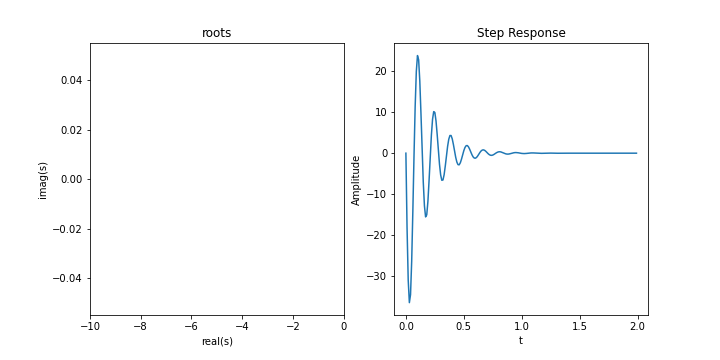
\includegraphics[scale=0.5]{fig1}
\FloatBarrier
\subsection*{(c)}
\end{document}